\section{Introduction}

To infer the current state of the body in space, the brain must rely on noisy sensory inputs. Thus, a degree of uncertainty in the reconstructed physical state is unavoidable. However, according to the rules of Bayesian inference, perceptual uncertainty can be reduced by combining overlapping information from different sensory modalities, weighting each signal in proportion to its reliability \cite{knill2004,kording2004,angelaki2008}. For example, psychophysical studies have shown that human observers behave optimally when integrating visual--proprioceptive \cite{vanbeers1999}, visual--haptic \cite{ernst2002}, or visual--auditory \cite{alais2004} cues. In these studies, the approach was to estimate noise levels of the two sensory modalities in separate unimodal experiments that were then used to predict performance in the bimodal case. Unfortunately, such a forward approach is difficult to implement when the involved sensory modalities cannot be studied in isolation, as in spatial orientation, which involves visual, somatosensory, and vestibular cues. Here the visual contribution can be eliminated easily, but to test whether somatosensory and vestibular cues are combined optimally, one cannot simply ``switch off'' one system to assess the noise level of the other. 

Instead, we took optimality as a starting point and implemented an inverse probabilistic approach to deduce noise levels of the various individual sensors. We probed two spatial orientation estimates---body-in-space and head-in-space orientation--- which, according to optimal theory, will use all available sensory signals that can be obtained by various reference frame transformations. This transformation and integration scheme, shown in Figure \ref{p1:fig1}, involves at least three sensory systems: (1) head sensors, supplying information about the orientation of the head with respect to gravity (vestibular system); (2) body sensors, providing an estimate of the orientation of the body in space (``somatic graviceptors'') \cite{mittelstaedt1997}; and (3) neck sensors, providing an estimate of the angle between head and body (neck proprioceptors). 

\begin{figure}
    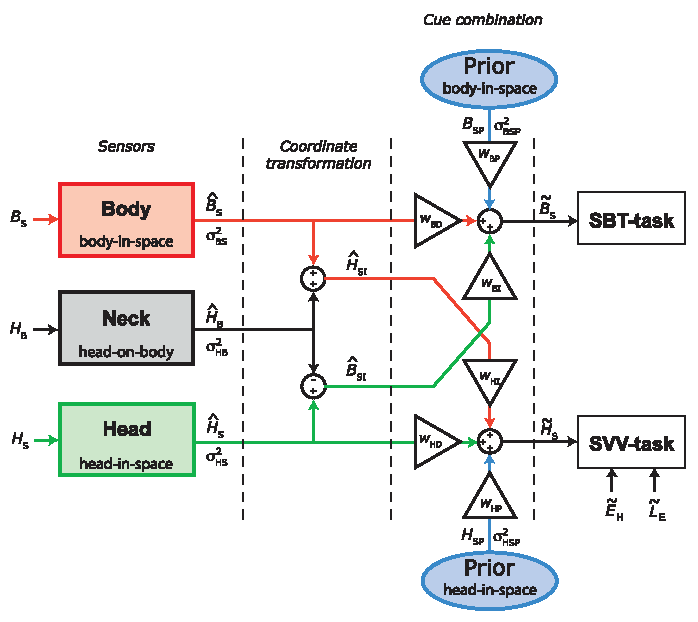
\includegraphics[width=0.75\textwidth]{src/paper1/figure1.pdf}
    
    \caption{Schematic representation of the sensory integration model. Sensory signals, denoted by a hat symbol (\textasciicircum), are assumed to be calibrated accurately, but contaminated by Gaussian noise. Optimal estimates are denoted by a tilde (\textasciitilde). Body sensors, neck sensors, and otoliths provide information about orientation of body in space ($B_S$), head on body ($H_B$), and head in space ($H_S$), respectively. Neck signal ($\hat{H}_B$) is used for a reference frame transformation of otolith information into a body-in-space signal ($\hat{H}_S - \hat{H}_B = \hat{B}_{SI}$), and for a transformation of body-tilt information into a head-in-space signal ($\hat{B}_S + \hat{H}_B = \hat{H}_{SI}$). For an optimal estimate of body-in-space orientation, $\tilde{B}_S$ (SBT task), the model combines the body-sensor signal ($\hat{B}_S$, red pathway) with a reference-frame-transformed otolith signal ($\hat{B}_{SI}$, green pathway). Relative contributions of the two pathways ($w_{BD}$ and $w_{BI}$) depend on their relative precision (Eq. \ref{p1:eqn2}). The scheme shows a symmetrical arrangement with two priors, but there is ample reason to believe that their effects are not identical. The simplest explanation of current and previous SBT data (see \nameref{p1:sec:methods}, \nameref{p1:sec:sbt_computation}) indicates that the associated prior in this task is uniform, which implies that $w_{BP}$ can be ignored. In the SVV task, an optimal estimate of head-in-space ($\tilde{H}_S$) is obtained by integration of otolith information ($\hat{H}_S$, green pathway), reference-frame-transformed information from body sensors ($\hat{H}_{SI}$, red pathway), and a significant contribution from prior information ($H_{SP}$, blue pathway). Relative weights are denoted by $w_{HD}$, $w_{HI}$, and $w_{HP}$, respectively. Estimate of line-in-space orientation is obtained by combining $\tilde{H}_S$ and estimates of eye-in-head ($\tilde{E}_H$) and line-on-eye ($\tilde{L}_E$) orientation. Noise variance in body sensors ($\sigma^2_{BS}$), neck sensors ($\sigma^2_{HB}$), otoliths ($\sigma^2_{HS}$), and width of prior ($\sigma^2_{HSP}$) defines their relative weights (see \nameref{p1:sec:methods}). Otolith noise may depend on tilt angle (Eq. \ref{p1:eqn11}). Note that the process of sensory integration, denoted here by summation of weighted sensory signals, is equivalent to multiplication of the underlying probability distributions (Eqs. \ref{p1:eqn2} and \ref{p1:eqn6} and \nameref{p1:sec:appendix}).}
    \label{p1:fig1}
\end{figure}

In this scheme, an estimate of body orientation in space can be obtained directly from the body sensors, but also indirectly from the head-sensor signal, by subtracting the neck signal. Likewise, the estimate of head-in-space orientation can be obtained from the head sensors, but also through an indirect pathway, by combining the body-sensor signal with neck information. Importantly, as the two state estimates require different transformations, Bayesian theory predicts that the relative contribution of the sensory signals will differ as well \cite{mcguire2009}. Apart from the crucial role of sensory information, the scheme allows for the possibility that the estimates of the two orientation states can be further influenced by prior beliefs about sensory states. 

Here, we used two psychophysical tasks---subjective body tilt (SBT) and subjective visual vertical (SVV) to quantify the two orientation estimates in a group of healthy subjects. Using an inverse probabilistic approach, we obtained stable solutions for the noise properties of the involved sensor systems. Independent measurements of neck noise confirmed the levels predicted by the model. Forward model predictions based on these noise properties were consistent with previously published deficits of bilateral vestibular and paraplegic patients, which would be difficult to explain otherwise. Our results suggest that Bayesian integration of multisensory information explains the major task-dependent features in spatial orientation perception. 
